\renewcommand*{\arraystretch}{1.1}

\noindent\begin{tabularx}{17cm}{|p{1.95cm}|X|}
	\hline
	workload    & BI \\ \hline
%
	query       & 11 \\ \hline
%
	title       & Unrelated replies \\ \hline
	\multicolumn{2}{|c|}{ 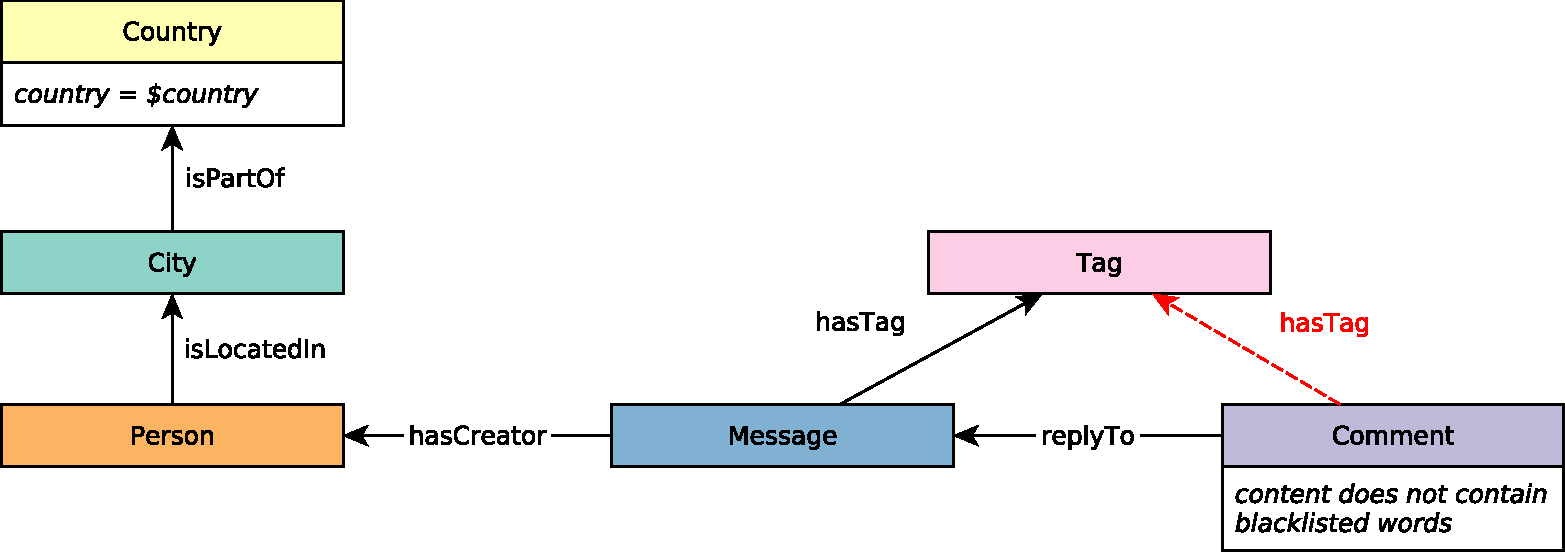
\includegraphics[scale=\patternscale,margin=0cm .2cm]{patterns/bi11}} \\ \hline
	description & Find those Persons of a given country that replied to any Message, such
that the reply does not have any Tag in common with the Message {[}are
transitive replies considered or not? - SzG{]}. Consider only those
replies not containing any word from a given blacklist. For each Person
and valid reply, retrieve the Tags associated with the reply, and
retrieve the number of likes on the reply.
 \\ \hline
	
%
	group by       &
	\multicolumn{1}{>{\raggedright}X|}{
		\varname{person.id}, 
		\varname{tag.name}
		} \\ \hline
	
%
	parameters  &
	\vspace{1.1ex}{\begin{tabularx}{14.38cm}{|c|M|m{2cm}|Y} \hline
	\cellcolor{black!70} \color{white} $\mathsf{1}$ & \varname{country} & \cellcolor{gray!20} \vartype{32-bit Integer} &  \\\hline
	\cellcolor{black!70} \color{white} $\mathsf{2}$ & \varname{blacklist} & \cellcolor{gray!20} \vartype{String[]} &  \\
	\end{tabularx}} \\ \hline
%
	result      &
	\vspace{1.1ex}{\begin{tabularx}{14.38cm}{|c|M|m{2cm}|Y} \hline
	\cellcolor{black!70} \color{white} $\mathsf{1}$ & \varname{person.id} & \cellcolor{gray!20} \vartype{64-bit Integer} &  \\\hline
	\cellcolor{black!70} \color{white} $\mathsf{2}$ & \varname{tag.name} & \cellcolor{gray!20} \vartype{String} &  \\\hline
	\cellcolor{black!70} \color{white} $\mathsf{3}$ & \varname{countLikes} & \cellcolor{gray!20} \vartype{32-bit Integer} & The count of Likes to replies with that Tag. \\\hline
	\cellcolor{black!70} \color{white} $\mathsf{4}$ & \varname{countReplies} & \cellcolor{gray!20} \vartype{32-bit Integer} & The count of replies with that Tag. \\
	\end{tabularx}} \\ \hline
	%
	sort        &
	\vspace{1.1ex}{\begin{tabular}{|c|l|c|} \hline
	\cellcolor{black!70} \color{white} $\mathsf{1}$ & \varname{countLikes} & \cellcolor{gray!20} $\desc$ \\\hline
	\cellcolor{black!70} \color{white} $\mathsf{2}$ & \varname{person.id} & \cellcolor{gray!20} $\asc$ \\\hline
	\cellcolor{black!70} \color{white} $\mathsf{3}$ & \varname{tag.name} & \cellcolor{gray!20} $\asc$ \\
	\end{tabular}} \\ \hline
	%
	limit       & 100 \\ \hline
	%
	choke points &
	\multicolumn{1}{>{\raggedright}X|}{
		\chokepoint{1.1}, 
		\chokepoint{2.1}, 
		\chokepoint{2.2}, 
		\chokepoint{2.3}, 
		\chokepoint{3.1}, 
		\chokepoint{3.2}, 
		\chokepoint{6.1}
		}\\ \hline
\end{tabularx}
\clearpage